\section{Matching games and the proposed method}\label{sec:method}

Both of the initialisation methods described in Section~\ref{subsec:inits} have
a greedy component. Cao's method essentially chooses the densest point that has
not already been chosen whilst forcing separation between the set of initial
modes. In the case of Huang's, however, the greediness only comes at the end
of the method, after the set of potential modes has been found by random
sampling.  In any practical implementation of this method, the order in which a
set of potential modes is iterated over has no guarantee of consistency. The
same is true for any arbitrary tie breaks. The result of this is that the
initial set of modes that the method returns is altered since the next initial
mode is chosen by the next locally optimal choice.

The initialisation method proposed in this work aims to extend Huang's method to
be order-invariant in the final allocation --- thereby eliminating its greedy
component --- and to provide a more intuitive starting point for the \(k\)-modes
algorithm. This is done by constructing and solving a matching game between the
set of potential modes and some subset of the data.

In general, matching games are defined by two sets (parties) of players (often
termed suitors and reviewers) in which each player creates a preference list of
at least some of the players in the other party. The objective then is to find a
mapping between the two sets of players such that no pair of players is
(rationally) unhappy with their matching. Such a mapping is considered stable.
Algorithms to find stable matchings to instances of matching games are often
structured to be party-oriented and aim to maximise some form of social or
party-based optimality~\cite{Fuku2006,Gale1962,Kwanashie2015}.

One of the simplest matching games models the Stable Marriage Problem (SM). In
this game the sets of players must be of equal size and rank each other strictly
(i.e.\ no ties allowed) and entirely. An algorithm was presented in the seminal
work by D.\ Gale and L.\ Shapley~\cite{Gale1962} that `solves' any instance of
SM by finding for it a unique, suitor-optimal, stable matching. This kind of
game is not considered in this work as it effectively reduces down to Huang's
method. This can be seen as follows. Note that the concept of preference between
points in an attribute space is synonymous with similarity. Thus, when
constructing the game, each potential mode gets to pick the data point it is
closest to but that has not already been picked. Then, up to an arbitrary
breaking of any ties in the preference lists, each potential mode is assigned to
its chosen data point.

A number of issues arise from this particular model other than it reducing to
Huang's method. For instance:
\begin{itemize}
    \item Ties are common when using the distance metric defined
        in~(\ref{eq:dissim}).
    \item There is no intuitively concrete way of constructing sets of players
        or their preference lists.
\end{itemize}

Allowing for ties is a simple extension to SM but the notion of stability
becomes tiered~\cite{Manlove1999}. In each case of stability, if such a matching
exists, then a polynomial-time algorithm will find one that is optimal for one
set of players. However, there is no guarantee that such a level-of-stable
matching exists and even in that case, the notion of party-optimality is
lost~\cite{Erdil2017}. Therefore this extension is not considered here where a
stable solution to the game is required, and is preferably party-optimal.

Further to allowing ties, how preference lists are constructed is a point of
interest in many applications of matching games~\cite{Iwama2008}. Often this is
a contextual problem and may be addressed in a number of ways. As in this case,
where similarity and preference are considered equivalent, a bespoke distance
metric may be used. Though not relevant to this work, if the game forms part of
a larger, long-standing or otherwise complex model, introducing flexibility in
preferences~\cite{Agarwal2017,Menzel2015} or estimating them
\emph{ad~hoc}~\cite{Rastegari2016} may be helpful to obtain meaningful
matchings.

Another method used to construct preference lists is to discount the preference
lists presented by players. For instance, where acceptability of another player
is the only criterion, binary preferences (i.e.\ incomplete preference lists
with ties) can create games that are invulnerable to manipulative players'
strategies~\cite{Bogomolnaia2004}. This approach can be adapted to cater for
larger games, such as student-school allocation. In this case, each student
submits a set of acceptable schools and the schools form strict rankings of the
students. The result of this is a simpler game (in the practical sense) and a
reduction in the set of possible stable
matchings~\cite{Haeringer2014,Haeringer2019}.

As this particular case has no interactive element, and must guarantee a stable
matching (ideally with optimality), none of these extensions are used in the
proposed method. Instead, so as to keep the method as simple as possible within
these constraints, the game used will model an instance of the Hospital-Resident
Assignment Problem (HR) which was presented with SM as a practical solution to
the problem that gives it its namesake~\cite{Gale1962}.

Like SM, there exists an algorithm that can provide a unique, party-optimal,
stable matching to any instance of HR.\ The resident-optimal algorithm is
presented in Algorithm~\ref{alg:hospital_resident} and is adapted from the
original to take advantage of the structure of the game~\cite{Roth1984}. The
game used to model HR, its matchings, and its notion of stability are defined in
Definitions~\ref{def:game}~\--~\ref{def:blocking}. A summary of these
definitions in the context of the proposed \(k\)-modes initialisation is given
in Table~\ref{tab:components}.

\begin{definition}\label{def:game}
    Consider two distinct sets \(R, H\) and refer to them residents and
    hospitals. Each \(h \in H\) has a capacity \(c_h \in \mathbb{N}\) associated
    with them. Each player \(r \in R\) and \(h \in H\) has associated 
    with it a strict preference list of the other set's elements such that:
    \begin{itemize}
        \item Each \(r \in R\) ranks a non-empty subset of \(H\), denoted by
            \(f(r)\).
        \item Each \(h \in H\) ranks all and only those residents that have
            ranked it, i.e.\ the preference list of \(h\), denoted \(g(h)\), is
            a permutation of the set
            \(\left\{r \in R \ | \ h \in f(r)\right\}\). If no such residents
            exist, \(h\) is removed from \(H\).
    \end{itemize}

    This construction of residents, hospitals, capacities and preference lists
    is called a \emph{game} and is denoted by \((R, H)\).
\end{definition}

\begin{definition}\label{def:matching}
    Consider a game \((R, H)\). A \emph{matching} \(M\) is any mapping between
    \(R\) and \(H\). If a pair \((r, h) \in R \times H\) are matched in \(M\)
    then this relationship is denoted \(M(r) = h\) and \(r \in M^{-1}(h)\).

    A matching is only considered \emph{valid} if all of the following hold for
    all \(r \in R, h \in H\):
    \begin{itemize}
        \item If \(r\) is matched then \(M(r) \in f(r)\).
        \item If \(h\) has at least one match then \(M^{-1}(h) \subseteq g(h)\).
        \item \(h\) is not over-subscribed, i.e.\ \(\abs*{M^{-1}(h)} \leq c_h\).
    \end{itemize}

    A valid matching is considered \emph{stable} if it does not contain any
    blocking pairs.
\end{definition}

\begin{definition}\label{def:blocking}
    Consider a game \((R, H)\). Then a pair \((r, h) \in R \times H\) is said to
    \emph{block} a matching \(M\) if all of the following hold:
    \begin{itemize}
        \item There is mutual preference, i.e.\ \(r \in g(h)\) and \(h \in
            f(r)\).
        \item Either \(r\) is unmatched or they prefer \(h\) to \(M(r)\).
        \item Either \(h\) is under-subscribed or \(h\) prefers \(r\) to at
            least one resident in \(M^{-1}(h)\).
    \end{itemize}
\end{definition}

\begin{table}[htbp]
    \resizebox{\textwidth}{!}{%
    \begin{tabular}{lcr}
        \toprule%
        Object in \(k\)-modes initialisation & {} & Object in a matching game
        \\\midrule%
        Potential modes & {} & The set of residents
        \\
        Data points closest to potential modes & {} & The set of hospitals
        \\
        Similarity between a potential mode and a point & {} & Respective
        position in each other's preference lists
        \\
        The data point to replace a potential mode & {} & A pair in a matching
        \\\bottomrule
    \end{tabular}}
    \caption{A summary of the relationships between the components of the
             initialisation for \(k\)-modes and those in a matching game
             \((R, H)\).
    }\label{tab:components}
\end{table}

%\begin{example}\label{example:matching}
    Consider the following example with \(S = \{A, B, C\}\) and \(R = \{D, E,
    F\}\). We can visualise this matching game as a bipartite graph as in
    Figure~\ref{fig:matching_bipartite}. In this representation, an edge between
    two vertices indicates that they are matched by \(M\). Beside each node is 
    the name of the node and a complete ranking of its complementary set's 
    elements. We interpret these rankings as the values of our preference list 
    functions. Here, for instance, \(A\) would most prefer to be matched with 
    \(D\), then \(E\), and finally \(F\).
    
    \begin{figure}[h]
        \centering
        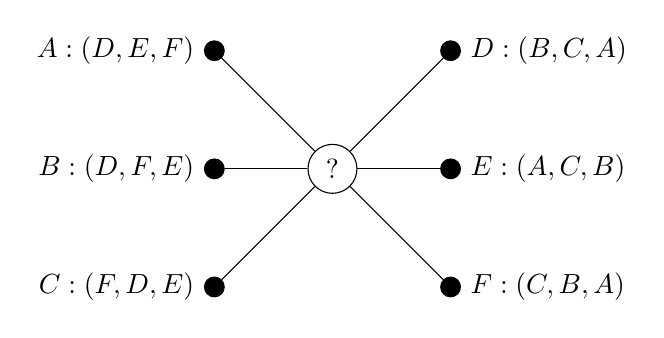
\begin{tikzpicture}[scale=0.5]

    % Suitors
    \node[draw, shape=circle, fill, inner sep=0, minimum size=0.25cm,
    label=left: {\(A: (D, E, F)\)}] (A) at (0, 0) {};
    \node[draw, shape=circle, fill, inner sep=0, minimum size=0.25cm, 
    label=left: {\(B: (D, F, E)\)}] (B) at (0, -3) {}; 
    \node[draw, shape=circle, fill, inner sep=0, minimum size=0.25cm, 
    label=left: {\(C: (F, D, E)\)}] (C) at (0, -6) {};

    % Reviewers
    \node[draw, shape=circle, fill, inner sep=0, minimum size=0.25cm, 
    label=right: {\(D: (B, C, A)\)}] (D) at (6, 0) {};
    \node[draw, shape=circle, fill, inner sep=0, minimum size=0.25cm, 
    label=right: {\(E: (A, C, B)\)}] (E) at (6, -3) {};
    \node[draw, shape=circle, fill, inner sep=0, minimum size=0.25cm,
    label=right: {\(F: (C, B, A)\)}] (F) at (6, -6) {};

    % Question mark node
    \node[draw, shape=circle] (q) at (3, -3) {?};
        
    % Lines into (?)
    \foreach \x in {A, B, C, D, E, F}
        \draw (\x) -- (q);

\end{tikzpicture}
\caption{A simple matching game represented on a bipartite
    graph.}\label{fig:matching_bipartite}

    \end{figure}

    Suppose we have the matching shown in Figure~\ref{fig:unstable_matching} for
    our game. This matching, \(M\) is valid since it is a bijection between 
    \(S\) and \(R\) but it is not stable. For instance, we have \((B, D)\) as a
    blocking pair since \(B\) would rather be matched with \(D\) than its 
    current match \(E\), and \(D\) would prefer to be matched with \(B\) than
    its current match \(A\).

    \begin{figure}[h]
        \centering
        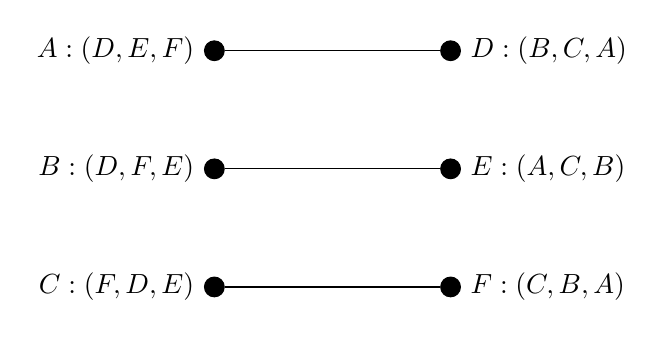
\begin{tikzpicture}[scale=0.5]

    % Suitors
    \node[draw, shape=circle, fill, inner sep=0, minimum size=0.25cm, 
    label=left: {\(A: (D, E, F)\)}] (A) at (0, 0) {};
    \node[draw, shape=circle, fill, inner sep=0, minimum size=0.25cm, 
    label=left: {\(B: (D, F, E)\)}] (B) at (0, -3) {}; 
    \node[draw, shape=circle, fill, inner sep=0, minimum size=0.25cm, 
    label=left: {\(C: (F, D, E)\)}] (C) at (0, -6) {};

    % Reviewers
    \node[draw, shape=circle, fill, inner sep=0, minimum size=0.25cm, 
    label=right: {\(D: (B, C, A)\)}] (D) at (6, 0) {};
    \node[draw, shape=circle, fill, inner sep=0, minimum size=0.25cm, 
    label=right: {\(E: (A, C, B)\)}] (E) at (6, -3) {};
    \node[draw, shape=circle, fill, inner sep=0, minimum size=0.25cm,
    label=right: {\(F: (C, B, A)\)}] (F) at (6, -6) {};

    % Lines
    \draw (A) -- (D);
    \draw (B) -- (E);
    \draw (C) -- (F);

\end{tikzpicture}
\caption{A example of an unstable matching for our
    game.}\label{fig:unstable_matching}

    \end{figure}

    We can make this matching stable by switching these pairs as in
    Figure~\ref{fig:stable_matching}. Here we have that each suitor is matched 
    with their most preferred reviewer so as not to form a blocking pair. We 
    call such a matching \emph{suitor-optimal}.

    \begin{figure}[h]
        \centering
        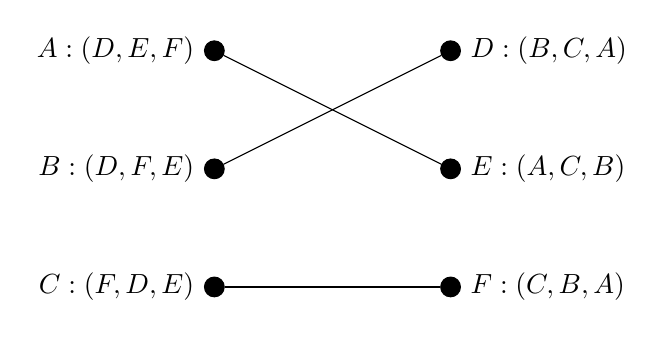
\begin{tikzpicture}[scale=0.5]

    % Suitors
    \node[draw, shape=circle, fill, inner sep=0, minimum size=0.25cm, 
    label=left: {\(A: (D, E, F)\)}] (A) at (0, 0) {};
    \node[draw, shape=circle, fill, inner sep=0, minimum size=0.25cm, 
    label=left: {\(B: (D, F, E)\)}] (B) at (0, -3) {}; 
    \node[draw, shape=circle, fill, inner sep=0, minimum size=0.25cm, 
    label=left: {\(C: (F, D, E)\)}] (C) at (0, -6) {};

    % Reviewers
    \node[draw, shape=circle, fill, inner sep=0, minimum size=0.25cm, 
    label=right: {\(D: (B, C, A)\)}] (D) at (6, 0) {};
    \node[draw, shape=circle, fill, inner sep=0, minimum size=0.25cm, 
    label=right: {\(E: (A, C, B)\)}] (E) at (6, -3) {};
    \node[draw, shape=circle, fill, inner sep=0, minimum size=0.25cm,
    label=right: {\(F: (C, B, A)\)}] (F) at (6, -6) {};

    % Lines
    \draw (A) -- (E);
    \draw (B) -- (D);
    \draw (C) -- (F);

\end{tikzpicture}
\caption{An example of a stable matching for our
    game.}\label{fig:stable_matching}

    \end{figure}
\end{example}


\balg%
    \caption{The hospital-resident algorithm
        (resident-optimal)}\label{alg:hospital_resident}
    \KwIn{a set of residents \(R\), a set of hospitals \(H\), a set of hospital
        capacities \(C\), two preference list functions \(f, g\)}
    \KwOut{a stable, resident-optimal mapping \(M\) between \(R\) and \(H\)}

    \For{\(h \in H\)}{%
        \(M^{-1}(h) \gets \emptyset\)
    }
    \While{There exists any unmatched \(r \in R\) with a non-empty preference
        list}{%
        Take any such resident \(r\) and their most preferred hospital \(h\)\;
        \(\textsc{MatchPair}(s, h)\)\;

        \If{\(\abs*{M^{-1}(h)} > c_h\)}{%
            Find their worst match \(r' \in M^{-1}(h)\)\;
            \(\textsc{UnmatchPair}(r', h)\)\;
        }
        \If{\(\abs*{M^{-1}(h)} = c_h\)}{%
            Find their worst match \(r' \in M^{-1}(h)\)\;
            \For{each successor \(s \in g(h)\) to \(r'\)}{%
                \(\textsc{DeletePair}(s, h)\)
            }
        }
    }
\ealg%

\balg%
    \caption{\textsc{MatchPair}}\label{alg:match}
    \KwIn{a resident \(r\), a hospital \(h\), a matching \(M\)}
    \KwOut{an updated matching \(M\)}

    \(M^{-1}(h) \gets M^{-1}(h) \cup \left\{r\right\}\)\;
\ealg%

\balg%
    \caption{\textsc{UnmatchPair}}\label{alg:unmatch}
    \KwIn{a resident \(r\), a hospital \(h\), a matching \(M\)}
    \KwOut{an updated matching \(M\)}

    \(M^{-1}(h) \gets M^{-1}(h) \setminus \left\{r\right\}\)\;
\ealg%

\balg%
    \caption{\textsc{DeletePair}}\label{alg:delete}
    \KwIn{a resident \(r\), a hospital \(h\)}
    \KwOut{updated preference lists}

    \(f(r) \gets f(r) \setminus \left\{h\right\}\)\;
    \(g(h) \gets g(h) \setminus \left\{r\right\}\)\;
\ealg%

\begin{algorithm}[H]
\caption{The proposed initialisation method}
    \begin{algorithmic}[0]
        \State{\textbf{Input:} a dataset \textbf{X}, with attribute sets \(A_1,
        \ldots, A_m\), and a number of modes to find \(k\)}
        \State{\textbf{Output:} a set of \(k\) initial modes \(\bar{\mu}\)\\}
        \\
        \Comment{Initialisation step}
        \State{\(\tilde{\mu} \gets \emptyset\)}
        \State{\(\bar{\mu} \gets \emptyset\)}
        \State{\(R \gets \emptyset\)}
        \State{\(S \gets \emptyset\)}
        \State{\(C \gets \{c_1, \ldots, c_k\}\)}

        \For{\(j = 1, \ldots, m\)}
            \For{\(s = 1, \ldots, d_j\)}
                \State{Calculate the relative frequency of each attribute value:
                    \(\frac{n(a_s^{(j)})}{N}\).}
	        \EndFor%
        \EndFor%
        \\
        \\
        \Comment{Find the set of virtual modes, \(\tilde{\mu}\), according to
        Huang's method.}
        \For{\(l = 1, \ldots, k\)}
            \For{\(j = 1, \ldots, m\)}
                \State{Consider the probability distribution given by:
                \(
                    \mathbb{P}(A_j) := \left(\frac{n(a_s^{(j)})}{N} : a_s^{(j)}
                    \in A_j\right)
                \)}
                \State{Sample \(a_{s^*}^{(j)}\) from \(A_j\) with respect to
                \(\mathbb{P}(A_j)\).}
                \State{\(\mu_j^{(l)} \gets a_{s^*}^{(j)}\)}
	        \EndFor%
            \State{\(\tilde{\mu} \gets \tilde{\mu} \cup
            \left\{\mu^{(l)}\right\}\)}
	    \EndFor%
        \\
        \\
        \Comment{Construct and solve a capacitated matching game.}
        \State{\(R \gets \tilde{\mu}\)}
        \For{\(r \in R\)}
            \State{\(c_r \gets 1\)}
            \State{Find the set of \(k\) vectors, \(S_r\), in \textbf{X} that 
            are the least dissimilar to \(r\).}
            \State{Arrange \(S_r\) into descending order of similarity.}
            \State{\(S \gets S \cup S_r\)}
        \EndFor%
        \For{\(r \in R\)}
            \State{\(g(r) \gets S_r\)}
        \EndFor%
        \State{Select a method for suitor preference lists and construct
        \(f(s)\) accordingly for each \(s \in S\).}
        \State{Solve the capacitated matching game defined by \((S, R, C)\) to
        obtain a matching \(M:~R~\to~S\).}
        \For{\(r \in R\)}
            \State{\(\bar{\mu} \gets \bar{\mu} \cup \{M(r)\}\)}
        \EndFor%
    \end{algorithmic}
\end{algorithm}

